\documentclass[a4paper,11pt,abstracton,hidelinks]{scrartcl}
\usepackage{dphil}
\usepackage{wasysym}
\addbibresource{refs.bib}
% hide section numbers
\setcounter{secnumdepth}{0}


\title{
Chapter 3. The \textit{Anopheles gambiae} 1000 Genomes Project phase 1 nucleotide variation data resource
}


\author{}


\begin{document}
\renewcommand{\abstractname}{Summary}


\maketitle



%%%%%%%%%%%%%%%%%%%%%%%%%%%%%%%%%%%%%%%%%%%%%%%%%%%%%%%%%%%%%%%%%%%%%%%%%%%%%%%
%%%%%%%%%%%%%%%%%%%%%%%%%%%%%%%%%%%%%%%%%%%%%%%%%%%%%%%%%%%%%%%%%%%%%%%%%%%%%%%
\begin{abstract}


In this chapter I describe the production and curation of a data resource of nucleotide variation obtained from whole-genome sequencing of 888 individual mosquitoes wild-caught from natural populations and a further 80 individuals from colony crosses.
%
Production of this data resource was a collaborative effort involving members of multiple research teams within the Ag1000G Consortium.
%
My contribution, described in this chapter, was to analyse the raw variant calls, define and carry out quality control and validation analyses, investigate genome accessibility and define quality filters, and produce the final analysis-ready data resource.
%
I also report analyses of these data to quantify the levels of nucleotide variation found, and to explore how genomic features such as protein-coding genes affect the genomic landscape of nucleotide variation.


\end{abstract}


\tableofcontents


%%%%%%%%%%%%%%%%%%%%%%%%%%%%%%%%%%%%%%%%%%%%%%%%%%%%%%%%%%%%%%%%%%%%%%%%%%%%%%%
%%%%%%%%%%%%%%%%%%%%%%%%%%%%%%%%%%%%%%%%%%%%%%%%%%%%%%%%%%%%%%%%%%%%%%%%%%%%%%%
\section{Introduction}


As described in chapter 1, the Ag1000G Project aims to use whole-genome deep Illumina sequencing to explore natural genetic variation among populations of malaria vectors within the \textit{An. gambiae} complex.
%
For logistical reasons the project was divided into three phases, and a total of 888 mosquito specimens sampled from natural populations were included in the first project phase.
%
A further 80 mosquito specimens comprising parents and progeny of four colony crosses were also sequenced within this project phase.
%
This chapter is primarily methodological, describing the processes and analyses developed and used to identify and genotype single nucleotide polymorphisms (SNPs) among these specimens.
%
For completeness, I have included some brief methodological information regarding population sampling and whole-genome sequencing which were performed by members of the Ag1000G Consortium.
%
However, the main focus of this chapter is the work I contributed to production and validation of a high quality genome-wide resource of SNP data from sequencing of these specimens.
%
Where work was carried out by or in collaboration with other members of the Ag1000G Consortium I have indicated that within the relevant subsection.



%%%%%%%%%%%%%%%%%%%%%%%%%%%%%%%%%%%%%%%%%%%%%%%%%%%%%%%%%%%%%%%%%%%%%%%%%%%%%%%
%%%%%%%%%%%%%%%%%%%%%%%%%%%%%%%%%%%%%%%%%%%%%%%%%%%%%%%%%%%%%%%%%%%%%%%%%%%%%%%
\section{Methods}


%%%%%%%%%%%%%%%%%%%%%%%%%%%%%%%%%%%%%%%%%%%%%%%%%%%%%%%%%%%%%%%%%%%%%%%%%%%%%%%
\subsection{Population sampling}


\begin{figure}[t!]
\centering
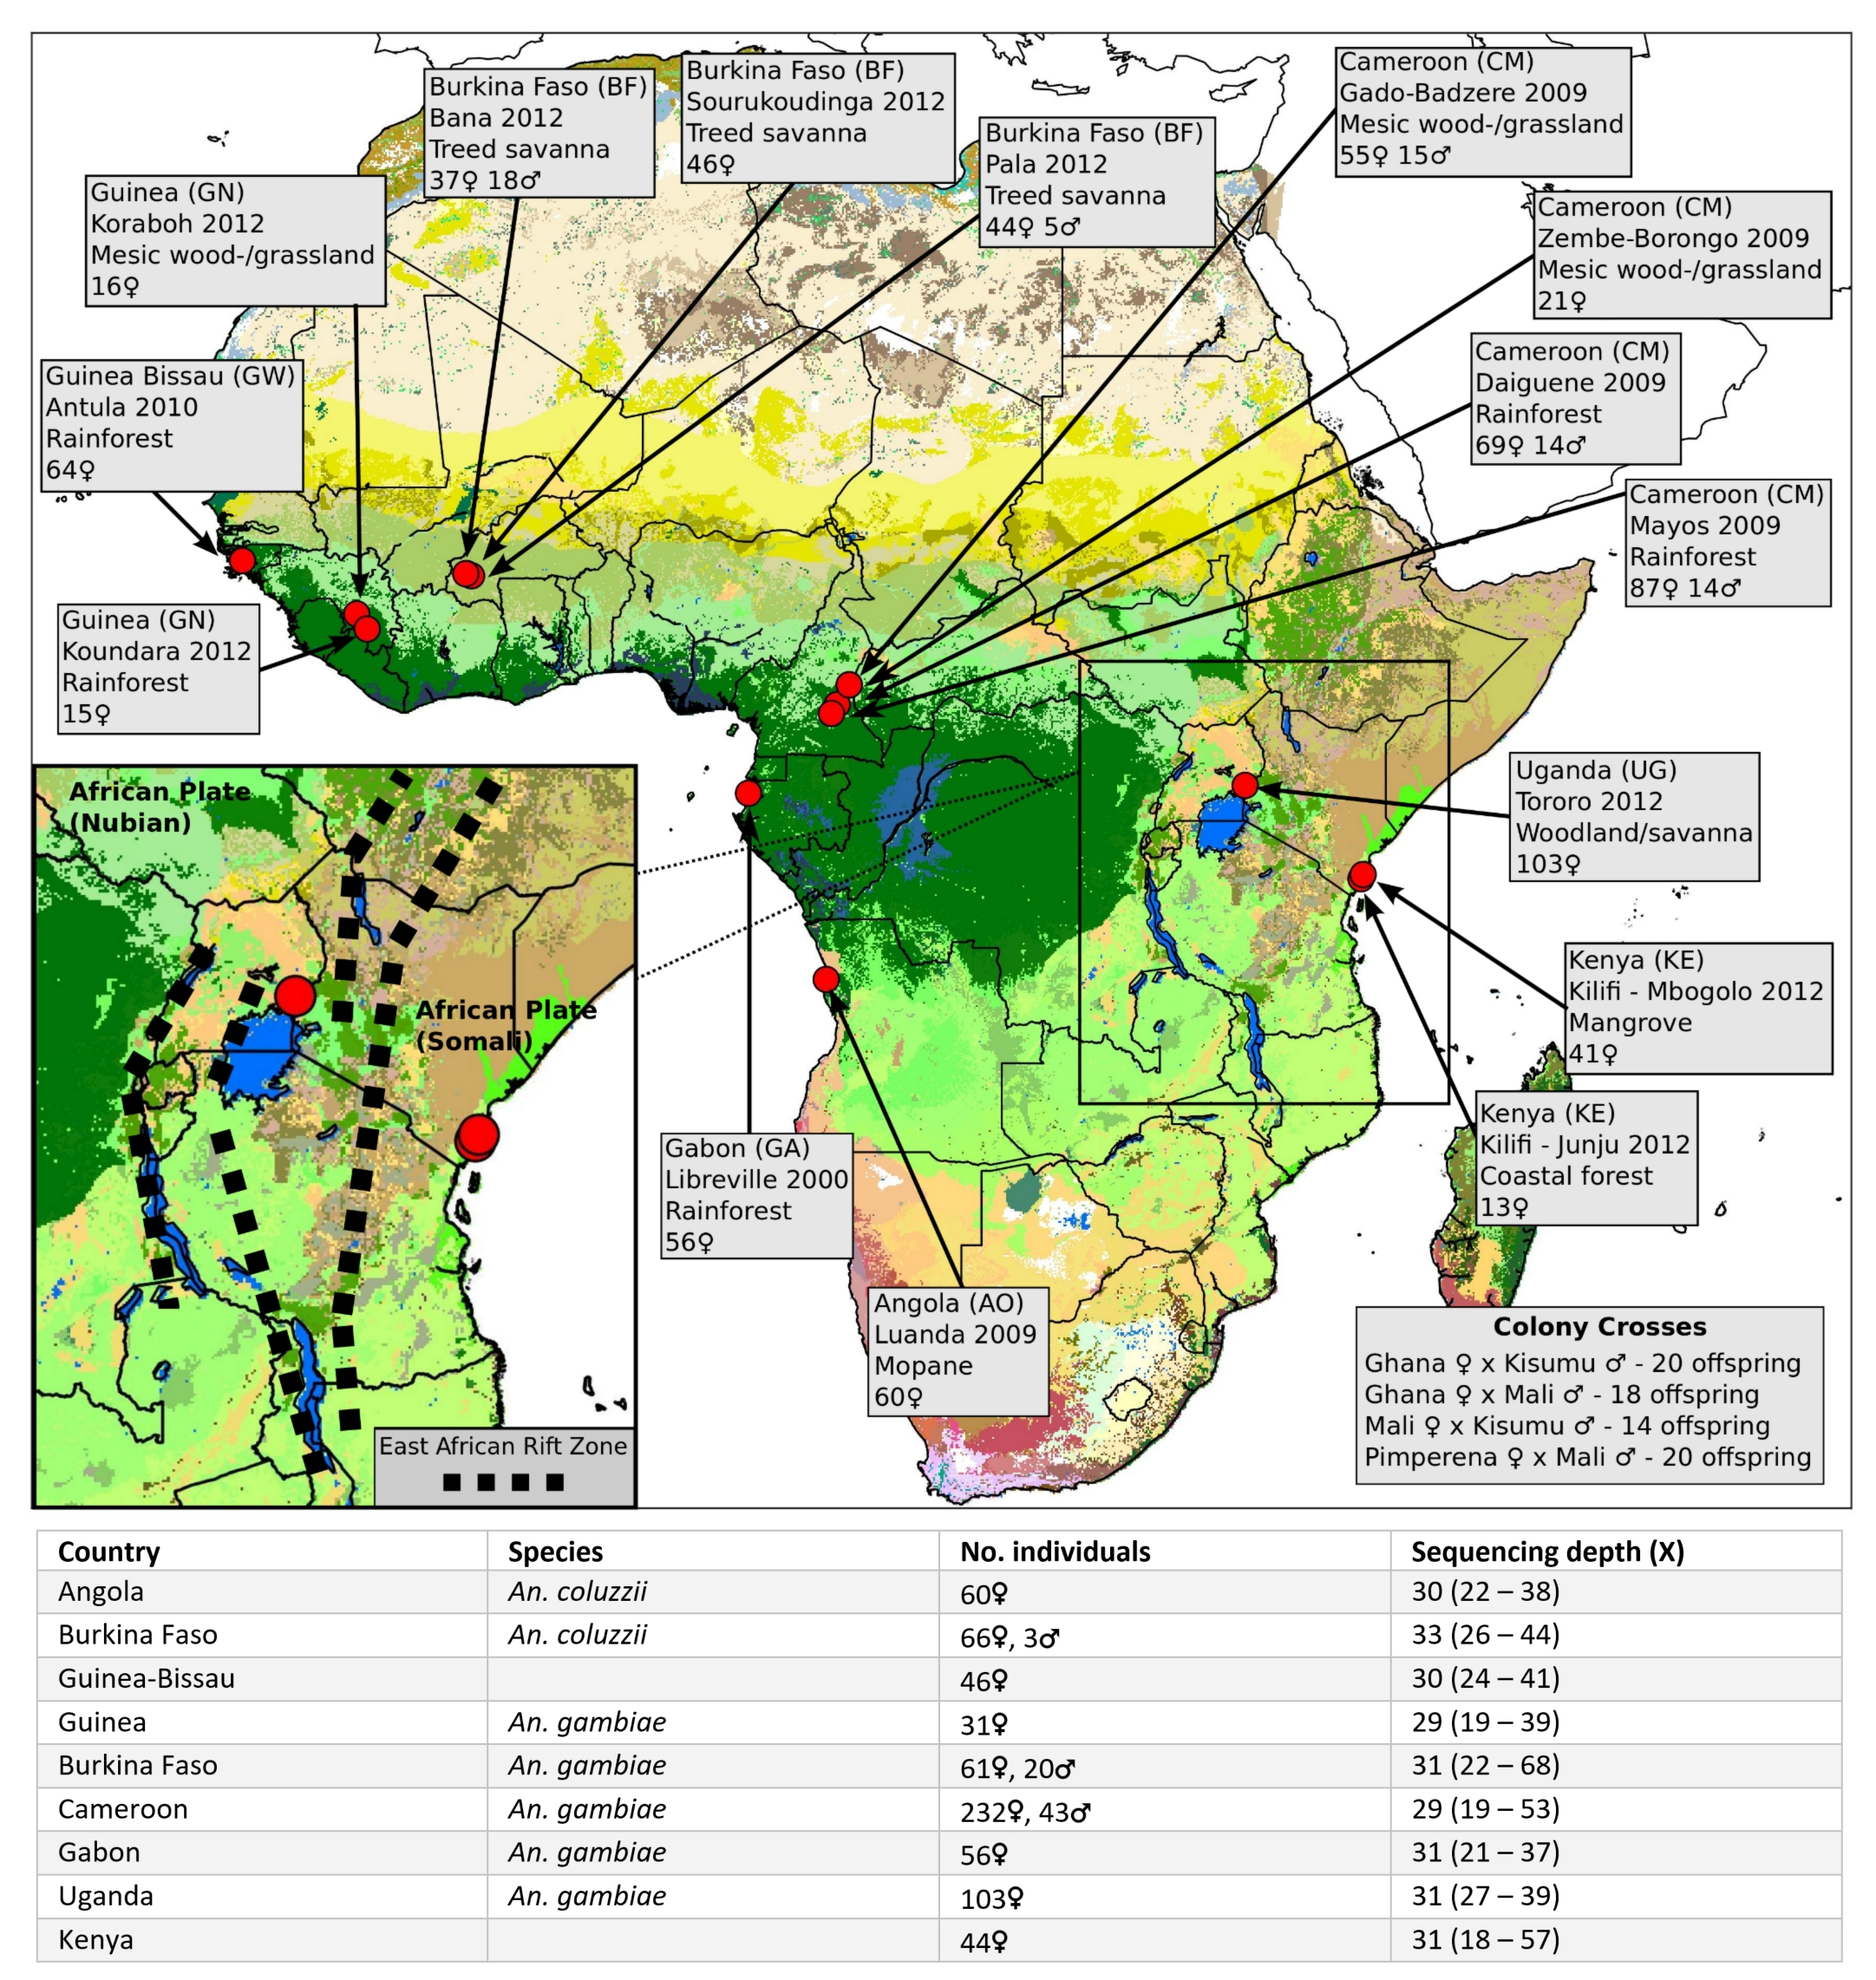
\includegraphics[width=\textwidth]{artwork/chapter3/map.jpeg}
\caption{Map of sampling locations and sample sizes.
%
Numbers of specimens are shown by gender.
%
Parental colonies and numbers of offspring for colony crosses are shown inset.
%
Numbers of samples are shown after all quality control steps described in this chapter were applied. 
%
@TODO explain colours. 
%
In the table below, the sequencing depth column shows the median (interquartile range) for the depth of coverage obtained for all samples, grouped by species and country of collection.
%
This figure was produced in collaboration with Chris Clarkson.}
\label{fig:map}
\end{figure}


\textit{Population sampling was performed by members of the Ag1000G Consortium. Below is a brief description of the cohort of mosquito specimens obtained for sequencing. A more detailed description is available in \citet{Ag1000G2017}.}


%%
A total of 888 mosquito specimens collected from natural populations were included in the Ag1000G phase 1 cohort.
%
This included mosquitoes representing two major malaria vector species  \textit{An. gambiae} and \textit{An. coluzzii}.
%
Mosquitoes were sampled from 8 countries in sub-Saharan Africa representing a broad geographical range spanning the continent: Guinea-Bissau, Guinea, Burkina Faso, Cameroon, Gabon, Angola, Uganda and Kenya (Fig. \ref{fig:map}).
%
Mosquitoes had been collected prior to the initiation of the Ag1000G Project as part of previous field studies, and were collected at different times, with the earliest collections being in 2000 (Gabon) and the most recent in 2012 (Burkina Faso).
%
Because these mosquitoes were collected in the context of different studies, a number of different collection methods were used, including light traps, pyrethrum spray catch and larval collection.
%
In addition to the wild-caught specimens, a further 80 mosquitoes were obtained from four colony crosses, each cross comprising two parents and up to 20 progeny, where parents were drawn from established reference colonies (Fig. \ref{fig:map} inset).
%
The main rationale for including colony crosses was to provide a mechanism for calibrating and measuring the accuracy of variant calling methods, because colony crosses allow for the analysis of genetic inheritance and Mendelian inconsistencies between parents and offspring, which can be a useful proxy of variant calling errors \citep{Saunders2007,Pilipenko2014}.
%
DNA extraction was performed on individual mosquitoes and genomic DNA samples were shipped to the Wellcome Sanger Institute for sequencing.


%%%%%%%%%%%%%%%%%%%%%%%%%%%%%%%%%%%%%%%%%%%%%%%%%%%%%%%%%%%%%%%%%%%%%%%%%%%%%%%
\subsection{Whole-genome sequencing}


\textit{Whole-genome sequencing was performed by staff at the Wellcome Sanger Institute sample logistics, sequencing and informatics facilities. Below is a brief description of sequencing methods. A more detailed description is available in \citet{Ag1000G2017}.}


%%
Sequencing was performed on the Illumina HiSeq 2000 platform at the Wellcome Sanger Institute.
%
Paired-end multiplex libraries were prepared using the manufacturer's protocol, with the exception that genomic DNA was fragmented using Covaris Adaptive Focused Acoustics rather than nebulization.
%
Multiplexes comprised 12 tagged individual mosquitoes and three lanes of sequencing were generated for each multiplex to even out variations in yield between sequencing runs.
%
Thus after sequencing data were demultiplexed, data for each individual sample were available from three separate sequencing runs.
%
Cluster generation and sequencing were undertaken per the manufacturer's protocol for paired-end 100 bp sequence reads with insert size in the range 100-200 bp.
%
Target coverage was $30\times$ per individual.
%
The median depth of coverage obtained per individual was between $29\times$ and $33\times$ depending on country (Fig. \ref{fig:map}).
%



%%%%%%%%%%%%%%%%%%%%%%%%%%%%%%%%%%%%%%%%%%%%%%%%%%%%%%%%%%%%%%%%%%%%%%%%%%%%%%%
%%%%%%%%%%%%%%%%%%%%%%%%%%%%%%%%%%%%%%%%%%%%%%%%%%%%%%%%%%%%%%%%%%%%%%%%%%%%%%%
\section{Results}


@TODO


%%%%%%%%%%%%%%%%%%%%%%%%%%%%%%%%%%%%%%%%%%%%%%%%%%%%%%%%%%%%%%%%%%%%%%%%%%%%%%%
%%%%%%%%%%%%%%%%%%%%%%%%%%%%%%%%%%%%%%%%%%%%%%%%%%%%%%%%%%%%%%%%%%%%%%%%%%%%%%%
\section{Conclusion}


@TODO


\section{Acknowledgments}


@TODO


\printbibliography


\end{document}
